
\begin{document}

\chapter{Studies}

\label{chapter:studies}

\section{Motivation}
\label{sec:studies_motivation}

A series of user studies are designed to evaluate the system's accuracy at tracking people in different scenarios. The accuracy of the tracking algorithm, or essentially the coordinate transformation algorithm, is measured by the differences in the joint coordinate between multiple potential skeletons of the same person. The studies will require participants to move around in front of multiple Kinects alone and with other participants. The software will log participants' positions from tracking, and these data will provide a quantitative feedback on the accuracy of the algorithm in different Kinect configurations and user scenarios.

To reiterate, a potential skeleton is a skeleton from a single Kinect field of view. One person may have multiple potential skeletons when they are visible to many Kinects. The application is most useful for its ability to transform any potential skeleton into any Kinect's camera space. The potential skeleton in the current Kinect field of view would be unaffected, but the other potential skeletons that were in other Kinects fields of view would have slight deviations in their joint coordinates. The user studies attempt to capture such deviations in all possible cases.

\section{Hypotheses}
\label{sec:studies_hypotheses}

The null hypotheses are:

\begin{enumerate}
  \item The differences in each joint coordinate among all potential skeletons of a person are consistent across time and are within five centimeters
  \item The differences in each joint coordinate among all potential skeletons of a person are consistent with different Kinect configurations
  \item The application would fill in the missing joint coordinates of a person from information about all potential skeletons
\end{enumerate}

\section{Apparatus}
\label{sec:studies_apparatus}

The current studies use two machines and two Kinects. Each machine is connected to one Kinect and runs a client sending Kinect BodyFrames to the server. The server is running on one of the client machines.

The server machine is running Microsoft Windows 8 on a i5-3470S CPU at 2.90 GHz and 8 Gb RAM . The other client machine is also running Microsoft Windows 8, on a i7-3610QM CPU at 2.30 GHz and 8 GB RAM.

The sensors are the v2 Kinects for Xbox One. The SDK running those Kinects is version 2.0.1410.19000.

\section{Participants}
\label{sec:studies_participants}

Participants are multinational university students and staff. There are participants in both genders and with a wide range of heights and weights. They are compensated with chocolates for participation.

\section{Setting}
\label{sec:studies_settings}

The studies take place in a semi-controlled environment (See Figure \ref{fig:studies_setting}). The two Kinects are placed at either three pre-defined locations, where they are approximately parallel, 45 and 90 degrees apart. One Kinect is always placed at the front position; it is the Kinect on the left in the image. (\textbf{(todo: measure the exact angles and distances between them - they are marked by duct tapes so shouldn't be too hard)}) Duct tapes are used to mark the precise locations of the Kinects. The boundary within which the participants will be moving is also marked with duct tapes. The sides of the block are found empirically to be near the minimum distance of the Kinect viewing range of the full body skeleton. The dimension of the boundary is x by x meters (\textbf{(todo: find the dimensions in meters)}). Each potential step is marked with duct tapes colored in a hue (either black or red) different from that on the duct tapes in the previous step. The starting position has a distinct color (green) from all other steps.

\begin{figure}[!h]
  \centering
  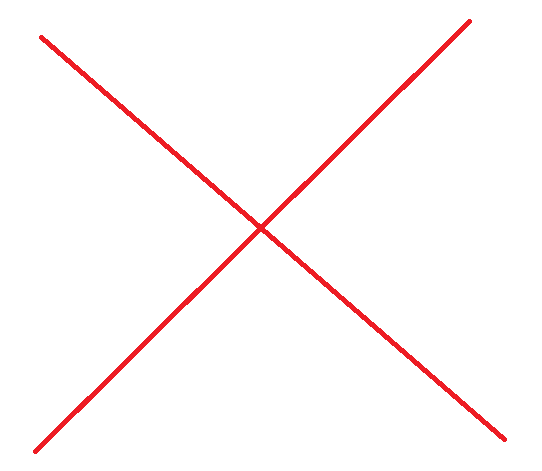
\includegraphics[width=0.5\linewidth]{figs/studies_setting}
  \caption{The setting where the user studies took place}
  \label{fig:studies_setting}
\end{figure}

\section{Method}
\label{sec:studies_method}

Firstly, participants are introduced to the project aims and objectives. They are given sufficient time to ask questions and decide whether to participate in the experiment before signing the consent form. Participants are free to withdraw from the studies at any time without any explanation. Secondly, participants are told beforehand what instructions they would expect during the experiments. This is because the studies are designed to measure how well the system tracks people, not how participants react to some situations. In user studies mode, the application would show instructions on the right hand side of the screen, telling the participants where to put their feet next. For instance, it would tell the participant to move forward (See Figure \ref{fig:studies_instruction}). The application will try to log as least amount of stationary movements as possible for tasks where they require participants to be moving. Not only because testing for differences in joint coordinates when the participant remains stationary is a standalone study, but also the researcher is interested in how the tracking algorithm performs when tracked people are constantly moving. To achieve this goal, the application introduces pauses between tasks. The researcher has control over the starting time of the next task. During the pauses, the researcher would give additional details about the studies to the participants.

\begin{figure}[!h]
  \centering
  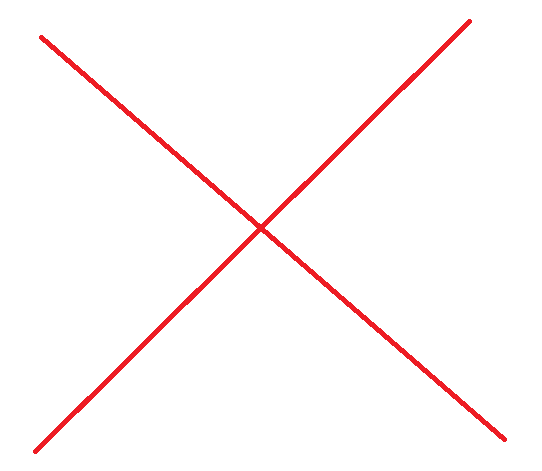
\includegraphics[width=0.5\linewidth]{figs/studies_instruction}
  \caption{Instructions during the user studies}
  \label{fig:studies_instruction}
\end{figure}

\section{Ethics}
\label{sec:studies_ethics}

There are no legitimate ethical concerns about participating in the studies. The skeleton data are anonymized and will be stored up to a maximum of three years. Any participant who feels uncomfortable with the guideline is welcome to speak to the researcher and his supervisor.

\section{Study 1: Stationary}
\label{sec:studies_stationary}

In the first study, participants are required to remain stationary for ten seconds in the center of the block. The study is done with all three Kinect configurations (Parallel, 45 degrees-apart and 90 degrees-apart)

\section{Study 2: Steps (Basic movements)}
\label{sec:studies_stationary}

The second study requires the participants to move in the same way as explained in the Wei et al study. These are basic movements such as moving forward, backward, left, and right. The study is done with all three Kinect configurations.

\section{Study 3: Walk (Continuous Movements)}
\label{sec:studies_stationary}

The third study requires the participants to walk around the perimeter of the block and walk diagonally to each of four corners. Like the previous two studies, study 3 is done with all three Kinect configurations. Studies 1, 2, 3 are conducted in succession for every participant.

\section{Study 4: Obstacle}
\label{sec:studies_stationary}

Participants are asked to walk around a large obstacle, which is a large poster in the current study. The obstacle divides the field of view of two Kinects at 90 degrees apart (See Figure \ref{fig:studies_obstacle}). The participant starts on the right hand side of the obstacle, where he is visible to both Kinects. As the participant walks around the obstacle, from the back, then to the left side of the obstacle, the Kinect that was looking at the side of the participant will slowly lose the sight of the person. When the participant is on the other side of the obstacle, only the front-facing Kinect will have sight of the person. The study should demonstrate that the system would still be able to track the person despite that one of the Kinect loses the person's sight temporarily. The study is only done with Kinects placed 90 degrees apart.

\begin{figure}[!h]
  \centering
  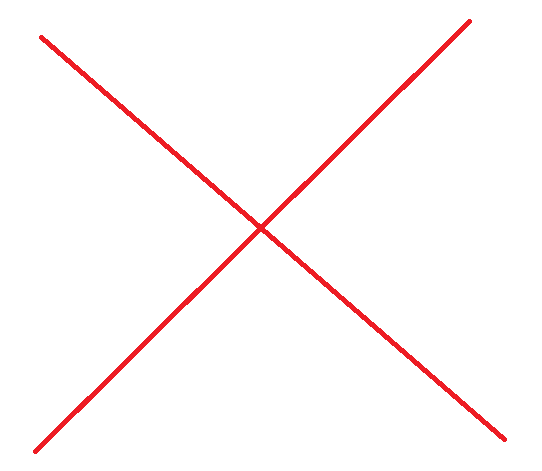
\includegraphics[width=0.5\linewidth]{figs/studies_obstacle}
  \caption{The obstacle in the actual experiment}
  \label{fig:studies_obstacle}
\end{figure}

\section{Study 5: Interaction}
\label{sec:studies_interaction}

The interaction study involves two people. They stand next to each other. The person on the left will walk to the front of the other person, then back to his initial position. Then he will walk around the person, from the front to the back, then return to his starting position. The other person does the same. In the end, both people exchange positions.

\end{document}
